% Inkling-turbo status figure.
%
% Build:  tectonic docs/figures/inkling_turbo_status.tex
% Render: pdftoppm -png -r 300 inkling_turbo_status.pdf status
%
% EVERY value is measured. Nothing is interpolated, estimated, or filled in.
% Source: one H100 SXM5 (sm_90), session 25, torch 2.11 / cu130.
%   journal/remote/microbench_attn_day0_session25_h100.json      (ours)
%   journal/remote/microbench_attn_scoremod_session25_h100.json  (day-0)
% A missing point means that pairing was never run.
%
% Design notes:
%  - A dot plot, not bars. On a log axis a bar's length is not proportional
%    to its value, so bars would misrepresent the ratios.
%  - Row guides come from the y grid, values from nodes near coords, row
%    names from yticklabels. No \foreach inside the axis: pgfplots replays
%    the axis body at \end{axis} and loop variables do not survive that.

\documentclass[border=12pt]{standalone}
\usepackage{tikz}
\usepackage{pgfplots}
\pgfplotsset{compat=1.18}
\usetikzlibrary{calc,plotmarks}

\definecolor{ours}{HTML}{0B6E6A}
\definecolor{floorc}{HTML}{64748B}
\definecolor{prod}{HTML}{C2410C}
\definecolor{altA}{HTML}{9A3412}
\definecolor{altB}{HTML}{78350F}
\definecolor{ink}{HTML}{111827}
\definecolor{guide}{HTML}{DCE0E5}
\definecolor{okc}{HTML}{15803D}
\definecolor{partc}{HTML}{B45309}

\begin{document}
\sffamily
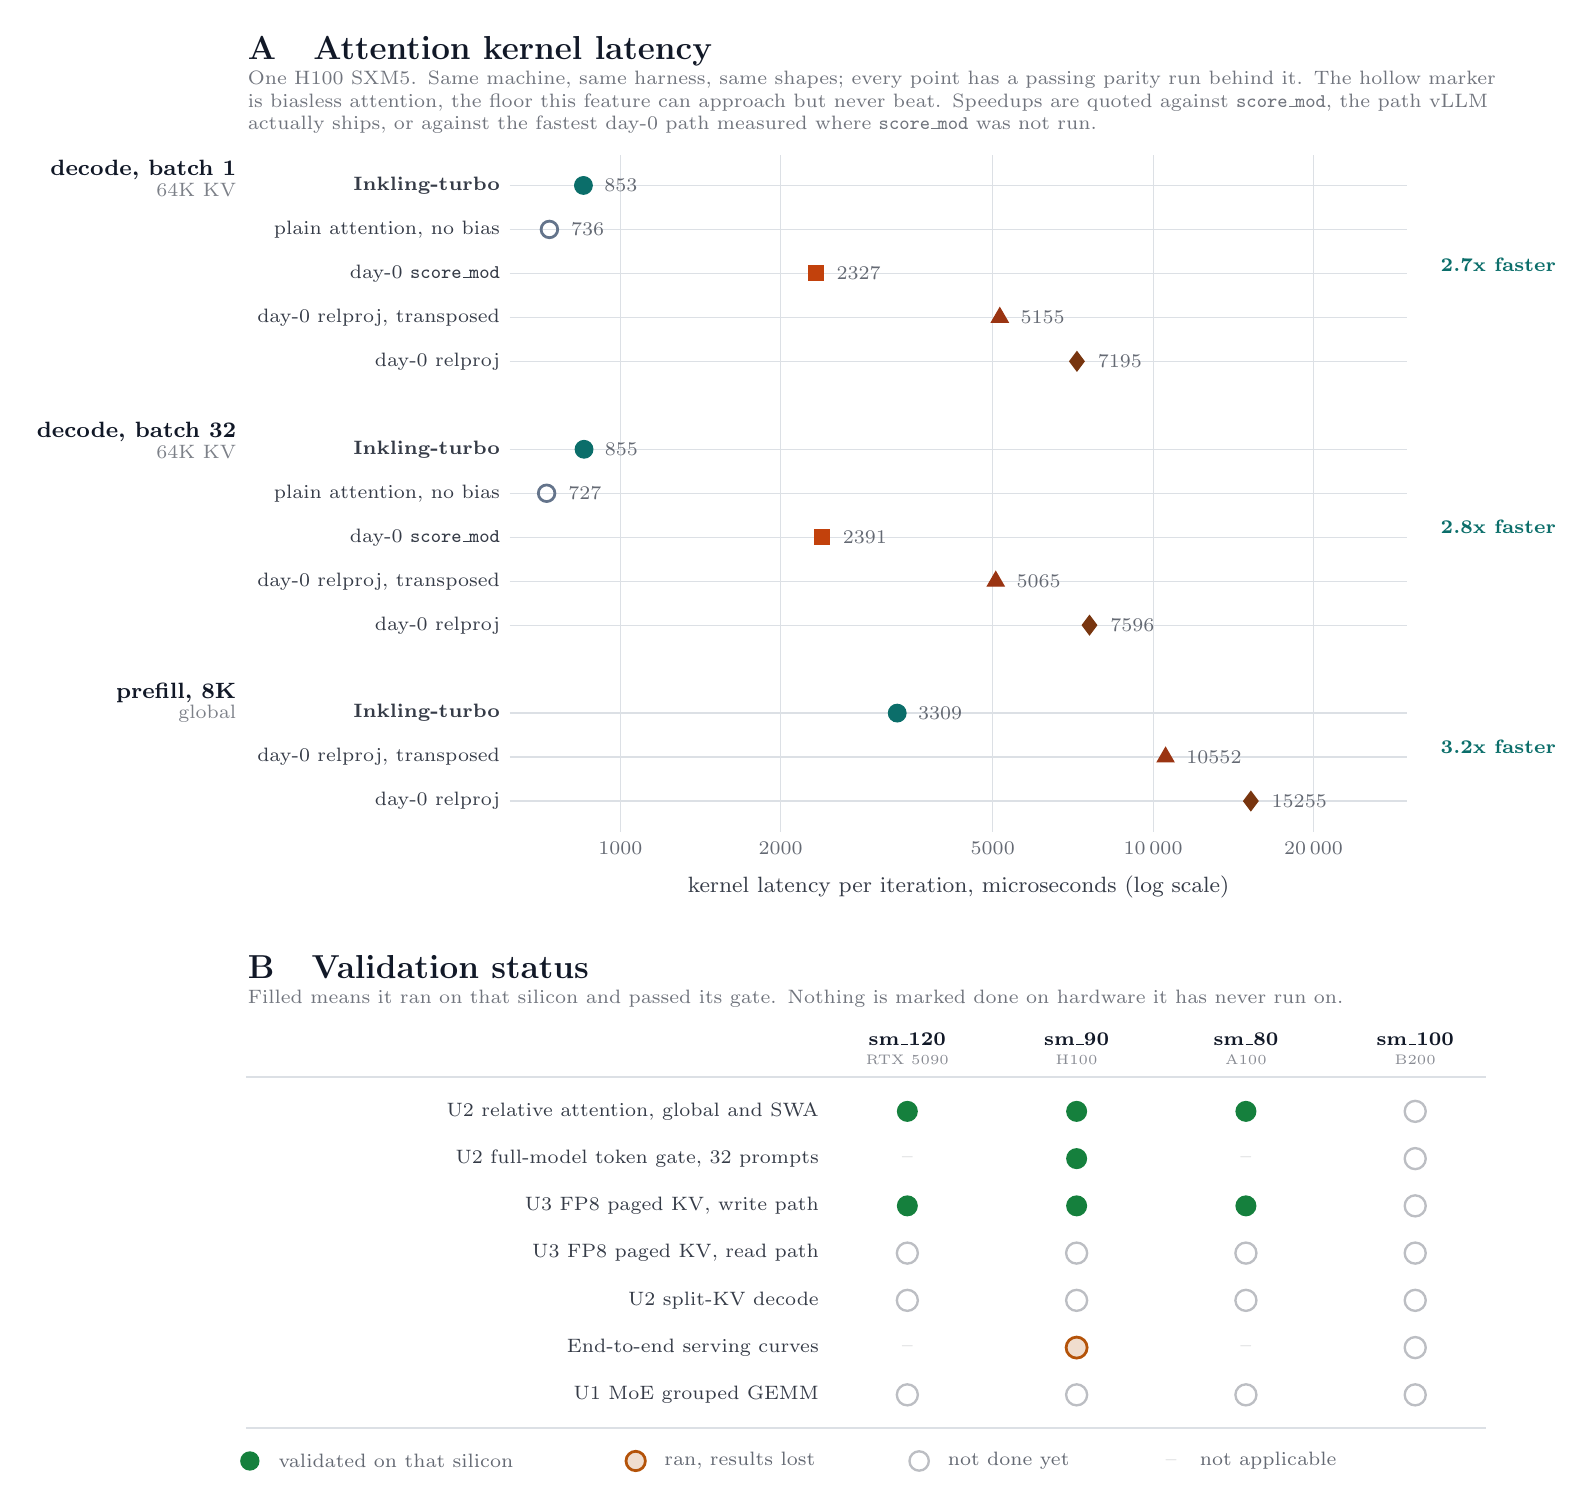
\begin{tikzpicture}[font=\sffamily]

% =====================================================================
% Panel A
% =====================================================================
\begin{axis}[
  name=A,
  width=11.4cm, height=8.6cm,
  scale only axis,
  xmode=log, log basis x=10,
  xmin=620, xmax=30000,
  xtick={1000,2000,5000,10000,20000},
  xticklabels={1000,2000,5000,{10\,000},{20\,000}},
  xlabel={kernel latency per iteration, microseconds (log scale)},
  xlabel style={font=\footnotesize, color=ink!85, yshift=-1pt},
  ymin=0.3, ymax=15.7,
  ytick={1,2,3,5,6,7,8,9,11,12,13,14,15},
  yticklabels={
    {day-0 relproj},
    {day-0 relproj, transposed},
    {\textbf{Inkling-turbo}},
    {day-0 relproj},
    {day-0 relproj, transposed},
    {day-0 \texttt{score\_mod}},
    {plain attention, no bias},
    {\textbf{Inkling-turbo}},
    {day-0 relproj},
    {day-0 relproj, transposed},
    {day-0 \texttt{score\_mod}},
    {plain attention, no bias},
    {\textbf{Inkling-turbo}}},
  yticklabel style={font=\scriptsize, color=ink!85},
  ymajorgrids, xmajorgrids,
  grid style={line width=0.45pt, color=guide},
  axis line style={draw=none},
  tick style={draw=none},
  xticklabel style={font=\scriptsize, color=ink!65},
  point meta=explicit symbolic,
  nodes near coords,
  nodes near coords style={font=\scriptsize, color=ink!65, anchor=west,
                           xshift=4pt},
  clip=false,
]

\addplot[only marks, mark=*, mark size=3.2pt, color=ours]
  coordinates {(852.6,15) [853] (854.8,9) [855] (3308.8,3) [3309]};

\addplot[only marks, mark=o, mark size=3.0pt, line width=1.0pt, color=floorc]
  coordinates {(736.0,14) [736] (727.2,8) [727]};

\addplot[only marks, mark=square*, mark size=2.7pt, color=prod]
  coordinates {(2326.6,13) [2327] (2391.2,7) [2391]};

\addplot[only marks, mark=triangle*, mark size=3.5pt, color=altA]
  coordinates {(5154.7,12) [5155] (5065.1,6) [5065] (10551.5,2) [10552]};

\addplot[only marks, mark=diamond*, mark size=3.5pt, color=altB]
  coordinates {(7194.5,11) [7195] (7595.5,5) [7596] (15254.6,1) [15255]};

\end{axis}

% ---- group headers, placed against the axis frame
\node[anchor=east, font=\footnotesize\bfseries, color=ink, align=right]
  at ($(A.north west)+(-3.35cm,-0.30cm)$)
  {decode, batch 1\\[-2pt]{\scriptsize\mdseries\color{ink!55}64K KV}};
\node[anchor=east, font=\footnotesize\bfseries, color=ink, align=right]
  at ($(A.north west)+(-3.35cm,-3.63cm)$)
  {decode, batch 32\\[-2pt]{\scriptsize\mdseries\color{ink!55}64K KV}};
\node[anchor=east, font=\footnotesize\bfseries, color=ink, align=right]
  at ($(A.north west)+(-3.35cm,-6.96cm)$)
  {prefill, 8K\\[-2pt]{\scriptsize\mdseries\color{ink!55}global}};

% ---- speedup callouts, quoted against the shipping path
\node[anchor=west, font=\scriptsize\bfseries, color=ours]
  at ($(A.north east)+(0.30cm,-1.40cm)$) {2.7x faster};
\node[anchor=west, font=\scriptsize\bfseries, color=ours]
  at ($(A.north east)+(0.30cm,-4.73cm)$) {2.8x faster};
\node[anchor=west, font=\scriptsize\bfseries, color=ours]
  at ($(A.north east)+(0.30cm,-7.52cm)$) {3.2x faster};

\node[anchor=north west, font=\bfseries, color=ink]
  at ($(A.north west)+(-3.45cm,1.62cm)$)
  {\large A\quad Attention kernel latency};
\node[anchor=north west, font=\scriptsize, color=ink!60, text width=16.3cm]
  at ($(A.north west)+(-3.45cm,1.18cm)$)
  {One H100 SXM5. Same machine, same harness, same shapes; every point has a
   passing parity run behind it. The hollow marker is biasless attention, the
   floor this feature can approach but never beat. Speedups are quoted against
   \texttt{score\_mod}, the path vLLM actually ships, or against the fastest
   day-0 path measured where \texttt{score\_mod} was not run.};

% =====================================================================
% Panel B
% =====================================================================
\begin{scope}[shift={($(A.south west)+(-3.45cm,-2.45cm)$)}]

\node[anchor=north west, font=\bfseries, color=ink] at (0,1.0cm)
  {\large B\quad Validation status};
\node[anchor=north west, font=\scriptsize, color=ink!60, text width=16.3cm]
  at (0,0.56cm)
  {Filled means it ran on that silicon and passed its gate. Nothing is marked
   done on hardware it has never run on.};

\def\cz{8.5}\def\cw{2.15}\def\rh{0.60}

\node[font=\scriptsize\bfseries, color=ink] at (8.50cm,-0.18cm) {sm\_120};
\node[font=\tiny, color=ink!50]             at (8.50cm,-0.44cm) {RTX 5090};
\node[font=\scriptsize\bfseries, color=ink] at (10.65cm,-0.18cm) {sm\_90};
\node[font=\tiny, color=ink!50]             at (10.65cm,-0.44cm) {H100};
\node[font=\scriptsize\bfseries, color=ink] at (12.80cm,-0.18cm) {sm\_80};
\node[font=\tiny, color=ink!50]             at (12.80cm,-0.44cm) {A100};
\node[font=\scriptsize\bfseries, color=ink] at (14.95cm,-0.18cm) {sm\_100};
\node[font=\tiny, color=ink!50]             at (14.95cm,-0.44cm) {B200};

\draw[guide, line width=0.6pt] (0.1cm,-0.66cm) -- (15.85cm,-0.66cm);

% state codes: 1 validated, 2 partial, 3 pending, 4 not applicable
\foreach \r/\name/\a/\b/\c/\d in {%
  0/{U2 relative attention, global and SWA}/1/1/1/3,
  1/{U2 full-model token gate, 32 prompts}/4/1/4/3,
  2/{U3 FP8 paged KV, write path}/1/1/1/3,
  3/{U3 FP8 paged KV, read path}/3/3/3/3,
  4/{U2 split-KV decode}/3/3/3/3,
  5/{End-to-end serving curves}/4/2/4/3,
  6/{U1 MoE grouped GEMM}/3/3/3/3%
}{
  \pgfmathsetmacro{\ry}{-1.10-\r*\rh}
  \node[anchor=east, font=\scriptsize, color=ink!85] at (7.5cm,\ry cm) {\name};
  \foreach \ci/\st in {0/\a, 1/\b, 2/\c, 3/\d}{
    \pgfmathsetmacro{\xx}{\cz+\ci*\cw}
    \ifnum\st=1
      \node[circle, fill=okc, minimum size=7.6pt, inner sep=0]
        at (\xx cm,\ry cm) {};
    \fi
    \ifnum\st=2
      \node[circle, draw=partc, fill=partc!20, line width=1.0pt,
            minimum size=7.6pt, inner sep=0] at (\xx cm,\ry cm) {};
    \fi
    \ifnum\st=3
      \node[circle, draw=ink!28, line width=0.85pt, minimum size=7.6pt,
            inner sep=0] at (\xx cm,\ry cm) {};
    \fi
    \ifnum\st=4
      \node[font=\scriptsize, color=ink!25] at (\xx cm,\ry cm) {--};
    \fi
  }
}

\draw[guide, line width=0.6pt] (0.1cm,-5.12cm) -- (15.85cm,-5.12cm);

\begin{scope}[shift={(0.15cm,-5.54cm)}]
  \node[circle, fill=okc, minimum size=7pt, inner sep=0] at (0,0) {};
  \node[anchor=west, font=\scriptsize, color=ink!65] at (0.24cm,0)
    {validated on that silicon};
  \node[circle, draw=partc, fill=partc!20, line width=1.0pt, minimum size=7pt,
        inner sep=0] at (4.9cm,0) {};
  \node[anchor=west, font=\scriptsize, color=ink!65] at (5.14cm,0)
    {ran, results lost};
  \node[circle, draw=ink!28, line width=0.85pt, minimum size=7pt, inner sep=0]
    at (8.5cm,0) {};
  \node[anchor=west, font=\scriptsize, color=ink!65] at (8.74cm,0)
    {not done yet};
  \node[font=\scriptsize, color=ink!25] at (11.7cm,0) {--};
  \node[anchor=west, font=\scriptsize, color=ink!65] at (11.94cm,0)
    {not applicable};
\end{scope}

\end{scope}
\end{tikzpicture}
\end{document}
